\section{Implementation and Results}
The algorithm is implemented in Java. 
We are currently performing experiments in order to evaluate the performance of the Rhone. 
%To perform this, a set of testcases have been produced varying the number of concrete services, CSDs, abstract services and measures. 
The figure~\ref{figure:chart1} is an example of the charts we have created.
In this example all the queries have 6 \textit{abstract services} and 2 \textit{single measures}. The number of local variables (dependencies) and CSDs is being modified to see how the algorithm works under these conditions.
\begin{center}
\begin{figure}[h!]
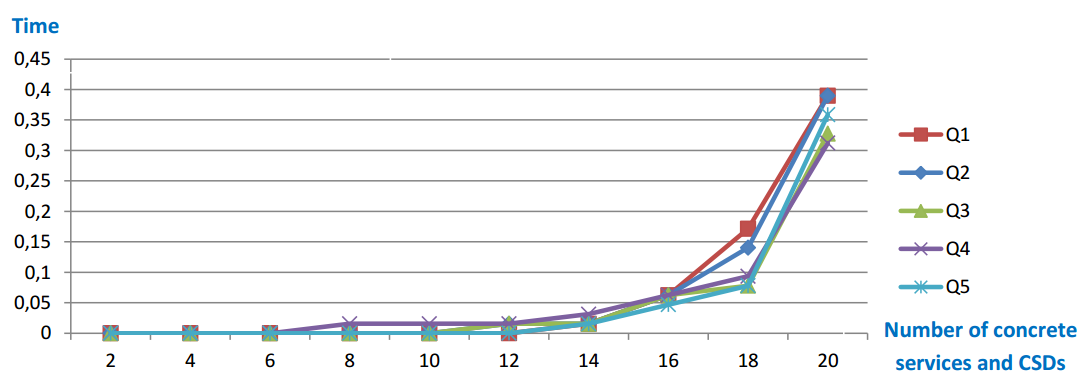
\includegraphics[scale=0.3]{chart1.PNG} 
\end{figure}\label{figure:chart1}
\end{center}

By now, the analysis identified that the factor that influenciates the Rhone performance is the number of CSDs vs. the number of abstract services in the query since they increase the number of possible combinations of CSDs.